% =====================================================================
%  main.tex — Manual de Defensa Personal para Mujeres
% =====================================================================

\documentclass[9pt, a5paper, twoside, openright]{extbook}

% =====================================================================
%  preamble.tex
%  Configuración global del documento: paquetes, idioma, estilo,
%  cajas destacadas y bibliografía.
%
%  Motor recomendado: pdflatex (compila también con xelatex/lualatex).
%  Bibliografía: BibTeX + natbib (estilo autor-año).
% =====================================================================

% ---------------------------------------------------------------------
%  Codificación y tipografía
% ---------------------------------------------------------------------
\usepackage[T1]{fontenc}      % Codificación de fuente moderna (acentos)
\usepackage[utf8]{inputenc}   % El fichero fuente está en UTF-8
% Latin Modern (fuentes vectoriales con buena cobertura de acentos).
% Se carga sólo si está disponible; en distribuciones completas y en
% Overleaf lo está. Si falta, se usa la Computer Modern por defecto.
\IfFileExists{lmodern.sty}{\usepackage{lmodern}}{}
% microtype: protrusion siempre; expansion=false evita el error fatal
% «auto expansion is only possible with scalable fonts» cuando, por
% falta de lmodern, se recurre a fuentes de mapa de bits.
\usepackage[protrusion=true, expansion=false]{microtype}
\usepackage{textcomp}         % Símbolos adicionales

% ---------------------------------------------------------------------
%  Idioma español
%  Se usa babel moderno con \babelprovide para no depender del antiguo
%  spanish.ldf. Aporta «Capítulo», «Índice», fechas y guiones en español.
% ---------------------------------------------------------------------
\usepackage{babel}
\babelprovide[import, main]{spanish}

% ---------------------------------------------------------------------
%  Geometría de página
% ---------------------------------------------------------------------
\usepackage[
  a4paper,
  top=2.6cm,
  bottom=2.6cm,
  inner=2.8cm,
  outer=2.4cm,
  headsep=14pt,
]{geometry}

% ---------------------------------------------------------------------
%  Color: paleta del manual
% ---------------------------------------------------------------------
\usepackage{xcolor}
\definecolor{primario}{HTML}{1F4E5F}   % Azul petróleo (títulos, filetes)
\definecolor{secundario}{HTML}{8E3B46} % Granate (acentos)
\definecolor{aviso}{HTML}{B23A48}      % Rojo aviso
\definecolor{consejo}{HTML}{2E7D5B}    % Verde consejo
\definecolor{regla}{HTML}{B07D2B}      % Ámbar regla de oro
\definecolor{grisclaro}{HTML}{F4F4F1}  % Fondo suave de cajas

% ---------------------------------------------------------------------
%  Listas, tablas y figuras
% ---------------------------------------------------------------------
\usepackage{enumitem}         % Control fino de listas
\setlist{itemsep=2pt, topsep=4pt, parsep=0pt}
\usepackage{booktabs}         % Filetes de tabla de calidad
\usepackage{tabularx}         % Tablas de ancho fijo
\usepackage{array}            % Mejoras en columnas
\usepackage{ragged2e}         % \RaggedRight en celdas
\usepackage{graphicx}         % Imágenes (carpeta figures/)
\graphicspath{{figures/}}

% ---------------------------------------------------------------------
%  Comillas (estilo español: «...»)
% ---------------------------------------------------------------------
\usepackage{csquotes}

% ---------------------------------------------------------------------
%  Cajas destacadas (avisos, consejos, definiciones)
% ---------------------------------------------------------------------
\usepackage[most]{tcolorbox}

% Caja genérica con título e icono textual
\newtcolorbox{cajadestacada}[2][]{%
  enhanced, breakable,
  colback=grisclaro, colframe=#2,
  boxrule=0.4pt, left=10pt, right=10pt, top=8pt, bottom=8pt,
  borderline west={3pt}{0pt}{#2},
  arc=2pt, fonttitle=\bfseries\color{#2},
  #1
}

% Aviso importante (rojo)
\newtcolorbox{aviso}{%
  enhanced, breakable,
  colback=aviso!6, colframe=aviso,
  boxrule=0.4pt, left=10pt, right=10pt, top=8pt, bottom=8pt,
  borderline west={3pt}{0pt}{aviso}, arc=2pt,
}

% Consejo (verde)
\newtcolorbox{consejo}{%
  enhanced, breakable,
  colback=consejo!6, colframe=consejo,
  boxrule=0.4pt, left=10pt, right=10pt, top=8pt, bottom=8pt,
  borderline west={3pt}{0pt}{consejo}, arc=2pt,
}

% Regla de oro (ámbar)
\newtcolorbox{reglaoro}{%
  enhanced, breakable,
  colback=regla!8, colframe=regla,
  boxrule=0.4pt, left=10pt, right=10pt, top=8pt, bottom=8pt,
  borderline west={3pt}{0pt}{regla}, arc=2pt,
}

% Definición / concepto (azul primario)
\newtcolorbox{definicion}{%
  enhanced, breakable,
  colback=primario!5, colframe=primario,
  boxrule=0.4pt, left=10pt, right=10pt, top=8pt, bottom=8pt,
  borderline west={3pt}{0pt}{primario}, arc=2pt,
}

% ---------------------------------------------------------------------
%  Estilo de títulos
% ---------------------------------------------------------------------
\usepackage{titlesec}

\titleformat{\chapter}[display]
  {\normalfont\sffamily\bfseries\color{primario}}
  {\filright\large\sffamily Capítulo \thechapter}
  {6pt}
  {\Huge}
  [\vspace{2pt}{\color{primario}\titlerule[1pt]}]
\titlespacing*{\chapter}{0pt}{10pt}{28pt}

\titleformat{\section}
  {\normalfont\sffamily\large\bfseries\color{primario}}
  {\thesection}{0.8em}{}
\titleformat{\subsection}
  {\normalfont\sffamily\bfseries\color{secundario}}
  {\thesubsection}{0.6em}{}

% ---------------------------------------------------------------------
%  Encabezados y pies de página
% ---------------------------------------------------------------------
\usepackage{fancyhdr}
\pagestyle{fancy}
\fancyhf{}
\renewcommand{\headrulewidth}{0.4pt}
\renewcommand{\footrulewidth}{0pt}
\fancyhead[LE]{\small\nouppercase{\leftmark}}
\fancyhead[RO]{\small\nouppercase{\rightmark}}
\fancyfoot[C]{\thepage}
% Estilo «plain» (primera página de capítulo) sólo con el número
\fancypagestyle{plain}{%
  \fancyhf{}\fancyfoot[C]{\thepage}%
  \renewcommand{\headrulewidth}{0pt}}

% ---------------------------------------------------------------------
%  Espaciado e interlineado
% ---------------------------------------------------------------------
\usepackage{setspace}
\setstretch{1.25}
\setlength{\parskip}{1.0em}
\setlength{\parindent}{0pt}
\usepackage{emptypage}        % Páginas en blanco realmente en blanco

% ---------------------------------------------------------------------
%  Bibliografía (autor-año con natbib + BibTeX)
% ---------------------------------------------------------------------
\usepackage[round, authoryear]{natbib}
\bibliographystyle{plainnat}
\setcitestyle{aysep={,}}

% ---------------------------------------------------------------------
%  Hiperenlaces y marcadores (cargar casi al final)
% ---------------------------------------------------------------------
\usepackage[
  colorlinks=true,
  linkcolor=primario,
  citecolor=secundario,
  urlcolor=secundario,
  pdftitle={Defensa Personal para Mujeres. Manual del Estudiante},
  pdfauthor={Artes Marciales Bilbao},
  pdfsubject={Manual de defensa personal y autoprotección},
]{hyperref}
\usepackage{bookmark}
\urlstyle{same}

% ---------------------------------------------------------------------
%  Comandos auxiliares
% ---------------------------------------------------------------------
% Teléfono/recurso destacado en línea
\newcommand{\recurso}[1]{\textbf{\color{primario}#1}}


% ----------------------------------------------------
% Compilar únicamente determinados capítulos
% ----------------------------------------------------
% \includeonly{chapters/01-introduccion}

\begin{document}

% ====================================================
% FRONT MATTER
% ====================================================

\frontmatter
\pagestyle{empty}

% ----------------------- Portada ---------------------
% =====================================================================
%  frontmatter/portada.tex — Página de título
% =====================================================================
\begin{titlepage}
\thispagestyle{empty}
\centering
\vspace*{\fill}

{\color{primario}\rule{\linewidth}{1.5pt}}\\[10pt]

{\sffamily\bfseries\fontsize{34}{38}\selectfont \color{primario}
DEFENSA PERSONAL\\[4pt] PARA MUJERES\par}

\vspace{10pt}
{\color{primario}\rule{\linewidth}{1.5pt}}\\[26pt]

{\sffamily\Large Manual del Estudiante\par}
\vspace{4pt}
{\large III Edición revisada y ampliada (2026)\par}

\vspace{30pt}
{\sffamily\large\color{secundario}
Prevención \textperiodcentered{} Actitud \textperiodcentered{} Técnica \textperiodcentered{} Recursos\par}

\vspace{\fill}

{\large\url{www.artesmarcialesbilbao.com}\par}
\vspace{10pt}
{\small Licencia Creative Commons BY-NC-SA 3.0 Unported\par}

\vspace*{\fill}
\end{titlepage}


% Páginas de cortesía iniciales (ajustar 0, 1 o 2 según cuadre el total).
% Van SIEMPRE de dos en dos si quieres mantener el índice en página impar.
% \paginacortesia
% \paginacortesia

% ----------------------- Índice ---------------------

\cleardoublepage
\pagestyle{plain}

\pdfbookmark[0]{Índice}{toc}
\tableofcontents

% ====================================================
% CUERPO DEL LIBRO
% ====================================================

\cleardoublepage
\mainmatter
\pagestyle{fancy}
\raggedbottom

% =====================================================================
%  Capítulo 1 — Introducción
% =====================================================================
\chapter{Introducción}
\citacap{En los campos de la observación, la suerte favorece únicamente a la mente preparada.}{Louis Pasteur}

El \textbf{objetivo} de este manual es lograr la mentalización necesaria para hacer frente a una situación en la que somos objeto de una agresión, potenciando nuestras habilidades y capacidades de defensa. Esta edición revisada está orientada específicamente a la mujer, e incorpora los avances de los últimos años en tres frentes: la evidencia científica sobre la eficacia de la autodefensa femenina, la actualización del marco legal español y las nuevas herramientas tecnológicas (aplicaciones móviles de seguridad ciudadana).

\textbf{La defensa personal NO es un arte marcial.} La mayoría de las artes marciales se han transformado en disciplinas competitivas donde se entrenan técnicas deportivas ---con sus normas--- en un ámbito protegido (monitores y árbitros). En la defensa personal el ambiente no es protegido y el objetivo es único: interrumpir la agresión y escapar.

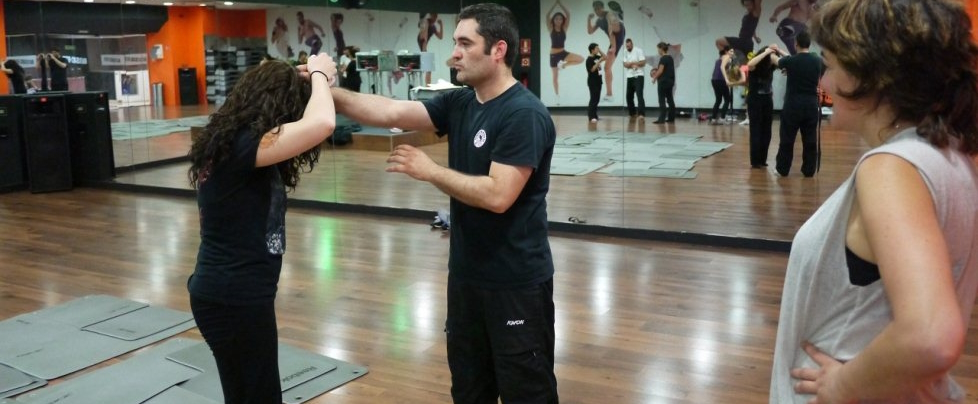
\includegraphics[width=\linewidth]{figures/02.jpg}

Dada la simplicidad de las técnicas de defensa personal, no se requieren años de práctica para poder aplicarlas. Pero debe quedar claro que la \enquote{magia} de las artes marciales consiste precisamente en la repetición de las técnicas infinidad de veces para que se interioricen y se expresen espontáneamente cuando sean necesarias. Esto es también aplicable a la defensa personal: las técnicas deberán practicarse y repasarse mentalmente hasta que su ejecución sea automática. Nadie puede esperar adquirir esta capacidad únicamente leyendo un manual.

La buena noticia es que hoy sabemos, con datos, que esto funciona. Un ensayo controlado aleatorizado publicado en el \emph{New England Journal of Medicine} \citep{senn2015} demostró que un programa de resistencia y autodefensa de 12 horas redujo en un 46\,\% el riesgo de violación consumada entre universitarias durante el año siguiente. Otros estudios \citep{hollander2014, sarnquist2014} confirman que el entrenamiento en autodefensa con enfoque de empoderamiento reduce la victimización y aumenta la confianza, sin trasladar la responsabilidad del delito a la víctima: la responsabilidad de una agresión es siempre, y únicamente, del agresor.

Se debe adquirir paulatinamente un pensamiento previsor de actitudes defensivas, aplicables ante ataques en los lugares que frecuentamos (imaginarnos qué haríamos si en la próxima esquina apareciese alguien que nos amenaza).

\textbf{En resumen:} no se trata solo de dominar unas técnicas de defensa, sino de prepararse mentalmente (atención y confianza) para una situación en la que debamos utilizarlas.

\begin{aviso}
\textbf{Aviso importante.} Este manual tiene fines educativos y no sustituye la formación presencial con instructores cualificados, ni el asesoramiento legal, médico o psicológico profesional. Si estás sufriendo violencia, en España puedes llamar al \recurso{016} (gratuito, 24\,h, no aparece en la factura) o al \recurso{112} en caso de emergencia.
\end{aviso}

% =====================================================================
%  Capítulo 2 — Estructura de un programa de defensa personal
% =====================================================================
\chapter{Estructura de un programa de defensa personal}

En la actualidad existen muchos sistemas de autoprotección, algunos con enfoque puramente técnico y otros con enfoque táctico. Encontraremos también sistemas que parten de enfoques específicos (policial, militar) que no son lo idóneo para la ciudadana común por las siguientes causas:

\begin{itemize}
  \item Quien creó el sistema y quien lo aprende no se enfrentan al mismo tipo de situaciones ni a agresores con los mismos objetivos.
  \item No suelen portar las mismas herramientas o armas.
  \item Tienen una predisposición y un entrenamiento psicológico muy distintos.
  \item Muchas técnicas van encaminadas a la contención, cuando lo que nos interesa es generar distancia para la interrupción y la huida.
  \item La legalidad para la que se pensó el sistema es diferente.
\end{itemize}

Esto no significa que no deban entrenarse esos sistemas, sino que deben considerarse ayudas para lograr la interrupción de la agresión y la huida.

Un sistema de autoprotección dirigido a civiles, asumiendo como objetivo la interrupción de la agresión y la huida del lugar, debería contener:

\begin{itemize}
  \item \textbf{Prevención y conciencia situacional} (el contenido más importante y el más rentable).
  \item \textbf{Habilidades verbales:} establecimiento de límites, desescalada, asertividad y uso de la voz.
  \item Bloqueos y cubiertas.
  \item Golpeos con armas corporales naturales (mano abierta, codo, rodilla, golpes bajos).
  \item Esquivas y desplazamientos.
  \item Agarres-sueltas y luxaciones simples.
  \item \textbf{Plan posterior:} huida, petición de ayuda, denuncia y autocuidado.
\end{itemize}

Todo ello trabajando desde distintas distancias: ambos de pie, pie-suelo, y ambos en el suelo.

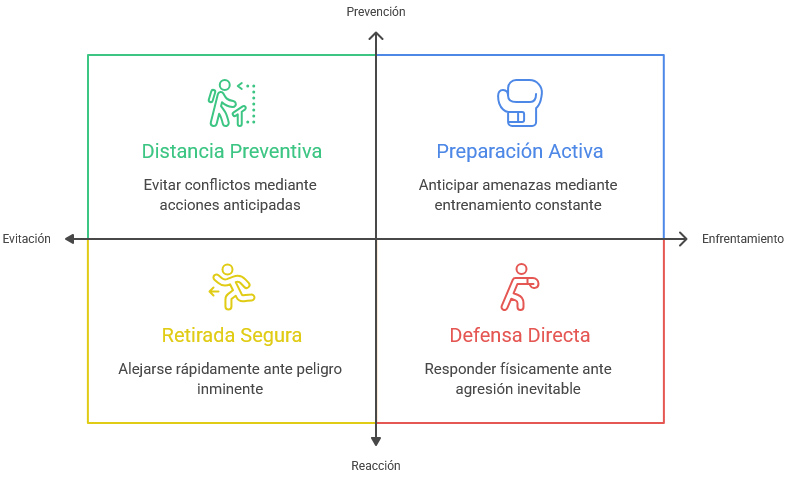
\includegraphics[width=\linewidth]{figures/evitacion.png}
% =====================================================================
%  Capítulo 3 — Actitud
% =====================================================================
\chapter{Actitud}
\citacap{La actitud es una pequeña cosa que marca una gran diferencia.}{Winston Churchill}

\begin{definicion}
\textbf{El \enquote{objetivo}} es el fin que se pretende alcanzar como resultado de una acción. El agresor tiene uno; nosotras, otro.

\medskip
\textbf{Las tácticas o estrategias} son las decisiones que se toman para que el objetivo llegue a cumplirse.

\medskip
\textbf{Las técnicas} son el conjunto de procedimientos y recursos concretos que se usarán. Generalmente tenemos inquietud por aprender técnicas, pero es mucho más importante tomar decisiones tácticas adecuadas.
\end{definicion}

Lo primero que hay que aclarar es que \textbf{no existen técnicas infalibles para todas las situaciones}. En el enfrentamiento real existen gran cantidad de variables que hacen única cada situación. Por eso entrenamos principios, no recetas.

Cuando hablamos de defensa personal nos referimos a un estado psicológico incorporado a nuestra rutina, caracterizado por una alerta relajada que, sin llegar a un comportamiento paranoico, permite una rápida reacción ante una situación de violencia.

\section{Niveles de atención (código de colores de Cooper)}

Un modelo clásico y útil para graduar nuestra atención es el código de colores popularizado por Jeff Cooper:

\begin{itemize}
  \item \textbf{Blanco:} desconexión total del entorno (auriculares a todo volumen, vista fija en el móvil). Es el estado que busca el agresor en su víctima. Evítalo en la calle.
  \item \textbf{Amarillo:} alerta relajada. Sé quién está a mi alrededor y qué pasa, sin tensión. Es el estado ideal y sostenible en espacios públicos.
  \item \textbf{Naranja:} algo concreto ha llamado mi atención (una persona, una situación). Evalúo, gano distancia, preparo opciones.
  \item \textbf{Rojo:} la amenaza se confirma. Ejecuto la decisión ya tomada: huir, pedir ayuda, defenderme.
\end{itemize}

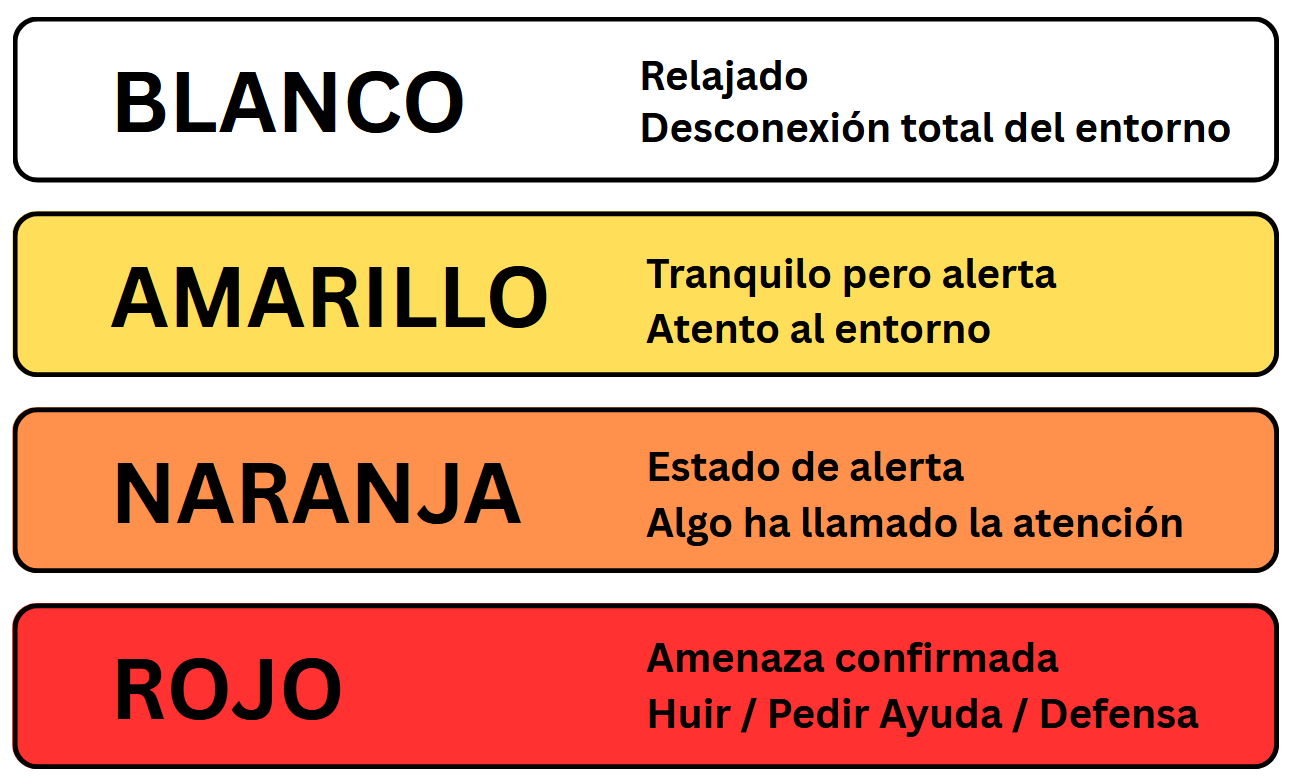
\includegraphics[width=\linewidth]{figures/cooper.png}

\section{La intuición es información}

La sensación de incomodidad o de \enquote{algo no va bien} ante una persona o lugar es un mecanismo de detección de señales reales que procesamos sin darnos cuenta (Gavin de Becker la describe en profundidad en su obra \emph{El valor del miedo}, \citeyear{debecker1997}). No la racionalices por cortesía: cambia de acera, no subas a ese ascensor, sal de ese portal. La educación social nos entrena para no \enquote{ofender}; \textbf{tu seguridad es más importante que la opinión de un desconocido}.

\section{Las tres distancias del conflicto}

\textbf{1) Distancia preventiva:} es la ideal para la defensa personal, ya que permite evitar el conflicto y no produce consecuencias. Si de noche debo pasar por un parque poco iluminado donde es común que se robe, hacer un rodeo por una calle iluminada y transitada me evita el riesgo. La defensa personal no se refiere solo a peleas: si evito esperar el metro muy cerca de las vías, estoy previniendo que alguien pueda empujarme (de manera intencionada o accidental).

\textbf{2) Distancia verbal o de negociación:} se establece cuando ya estamos inmersas en un conflicto. Todavía existe la posibilidad de disuadir al oponente y salir sin consecuencias. Lo siguiente en ocurrir suele depender en parte de los estímulos que lleguen al agresor.

\textbf{Debemos:}
\begin{itemize}
  \item Buscar la conciliación cuando el conflicto sea de baja intensidad (discusión, malentendido), intentando llegar a un acuerdo.
  \item Recordar al agresor las consecuencias (pérdida de tiempo o de prestigio, dolor, riesgo de ser detenido). Usar la técnica asertiva del \enquote{disco rayado}: repetir el mismo límite con las mismas palabras, sin entrar en provocaciones.
  \item Marcar límites con frases cortas, directas, en tono fuerte y con lenguaje corporal firme: \enquote{¡Para! ¡No te acerques!}. Verbalizar en voz alta también alerta a posibles testigos y rompe el guion del agresor, que espera una víctima callada.
\end{itemize}

\textbf{No debemos:}
\begin{itemize}
  \item Burlarnos, reírnos o ridiculizar al agresor.
  \item Insultarle.
  \item Iniciar el enfrentamiento con el lenguaje corporal.
  \item Sostener la mirada fija en los ojos de forma desafiante (sí mantenerlo en el campo visual).
  \item Tocar al agresor.
  \item Ignorarle por completo.
\end{itemize}

\textbf{3) Distancia física o de contacto:} puede llegar sin pasar por la distancia verbal, pero si deriva de esta, ya debemos haber recogido información del medio: cantidad de atacantes, vías de escape, elementos que puedan servir para la defensa, existencia de testigos, estado emocional del oponente, puntos vulnerables, etc.

\newpage

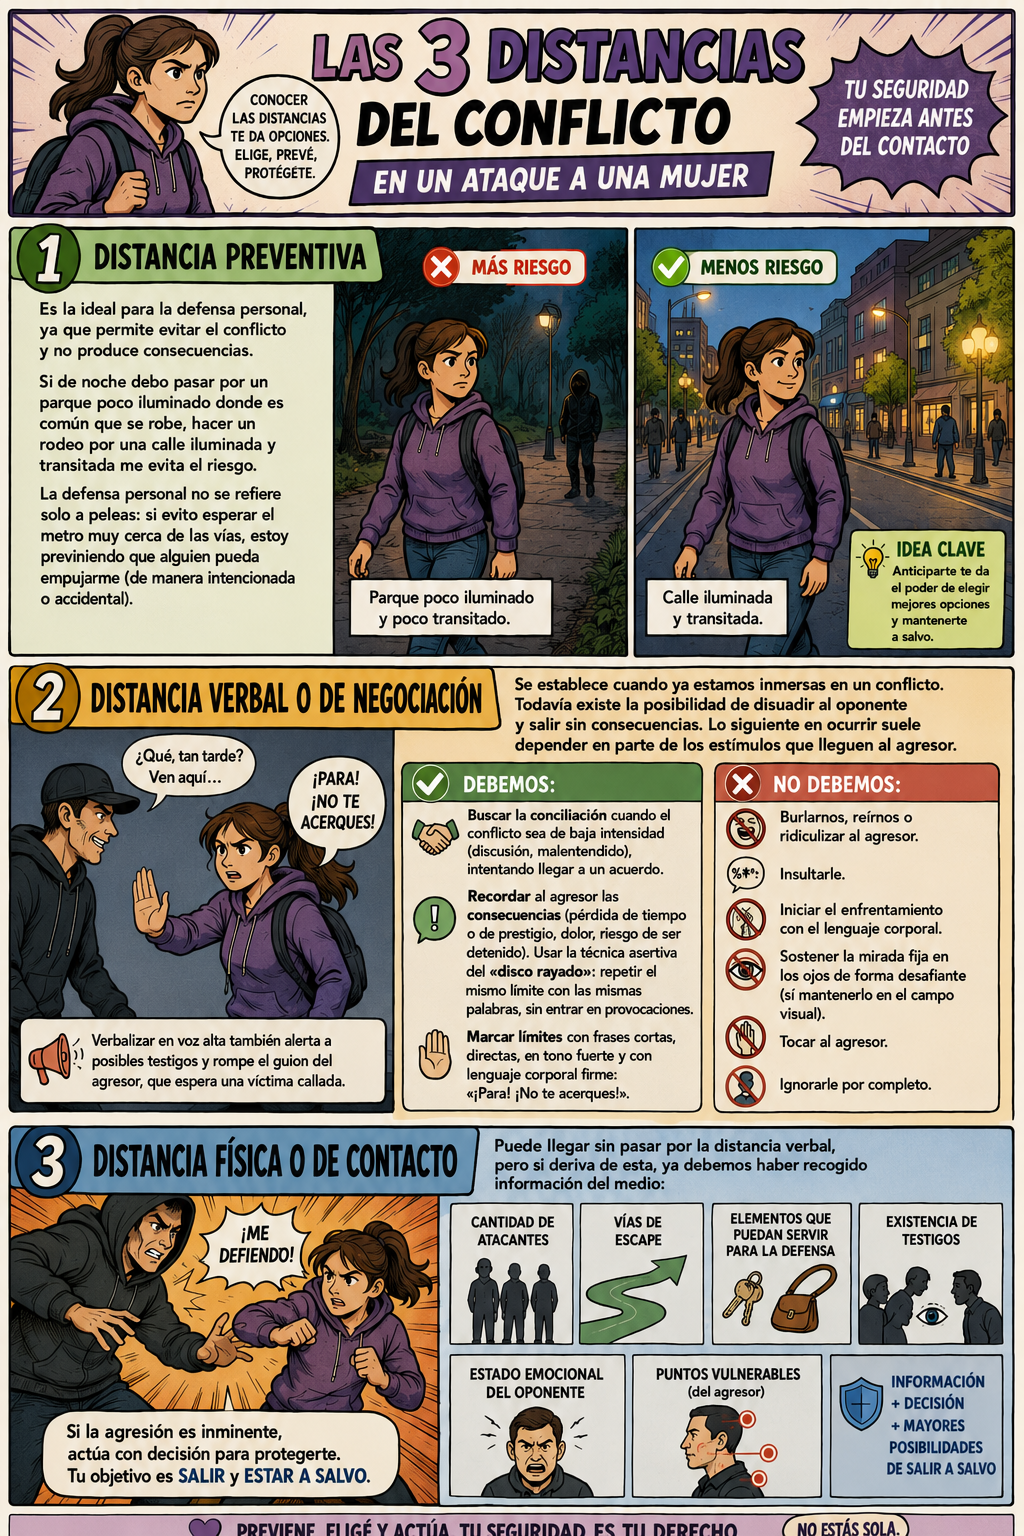
\includegraphics[width=\linewidth]{figures/tres-distancias.png}

% =====================================================================
%  Capítulo 4 — Cómo actuar
% =====================================================================
\chapter{Cómo actuar}
\citacap{Saber no es suficiente; debemos aplicar. Querer no es suficiente; debemos hacer.}{Johann Wolfgang von Goethe}

Los principios fundamentales dictan que toda respuesta de defensa personal debe ser:

\begin{itemize}
  \item Rápida
  \item Fuerte
  \item Natural
  \item Directa
\end{itemize}

La idea básica consiste en ocuparse primero de la amenaza inmediata (por ejemplo, un estrangulamiento), impedir que el agresor vuelva a atacar y, solo si es imprescindible, neutralizarle. Se hace énfasis en quitarle la iniciativa.

Es importante \textbf{anticiparse}: todo gesto físico tiene un \enquote{armado}, una \enquote{trayectoria} y un \enquote{impacto}, y con entrenamiento puede verse e interceptarse.

\section{La secuencia en un conflicto}

\begin{enumerate}
  \item \textbf{Cúbrete:} si el objetivo del agresor es pegarte, lo intentará hasta que se canse o algo lo detenga. Interesa cubrir cabeza, cuello y torso. Llevarse un golpe en brazos o piernas siempre será mejor que en la sien, la garganta o las costillas.
  \item \textbf{Anula su visión:} lanzando objetos a la cara del agresor, usando nuestras manos y dedos, escupiendo a los ojos, etc.
  \item \textbf{Gana tiempo} buscando su desequilibrio: empujón con una o ambas manos.
  \item \textbf{Huye:} correr sí, pero no en cualquier momento ni dirección. Antes del sprint hacia el punto de huida, coloca al agresor en una situación en la que no pueda interceptarte (movimiento obligado). Huye hacia luz, gente y ruido, nunca hacia zonas más aisladas.
\end{enumerate}

\section{Lucha, huida\ldots{} y parálisis: lo que dice la ciencia actual}

Ante un enfrentamiento se libera un torrente hormonal (adrenalina, cortisol) que prepara el organismo para combatir o emprender la fuga: visión en túnel, aumento de pulsaciones, pérdida de motricidad fina. Entrenar bajo estrés (con compañero, protecciones y escenarios) reduce estos efectos y nos enseña a operar con ellos.

Pero la investigación reciente ha confirmado una tercera respuesta involuntaria: la \textbf{inmovilidad tónica} o parálisis. Un estudio sueco con 298 supervivientes de violación \citep{moller2017} encontró que el 70\,\% experimentó inmovilidad significativa durante la agresión. Es una respuesta neurobiológica automática, no una decisión ni una forma de consentimiento. Esto tiene dos consecuencias prácticas: primero, si alguna vez te quedaste paralizada, no fue culpa tuya ni debilidad; segundo, el entrenamiento repetido y realista es precisamente la herramienta que más reduce la probabilidad de quedarse bloqueada, porque da al cerebro respuestas preprogramadas que ejecutar.

\newpage

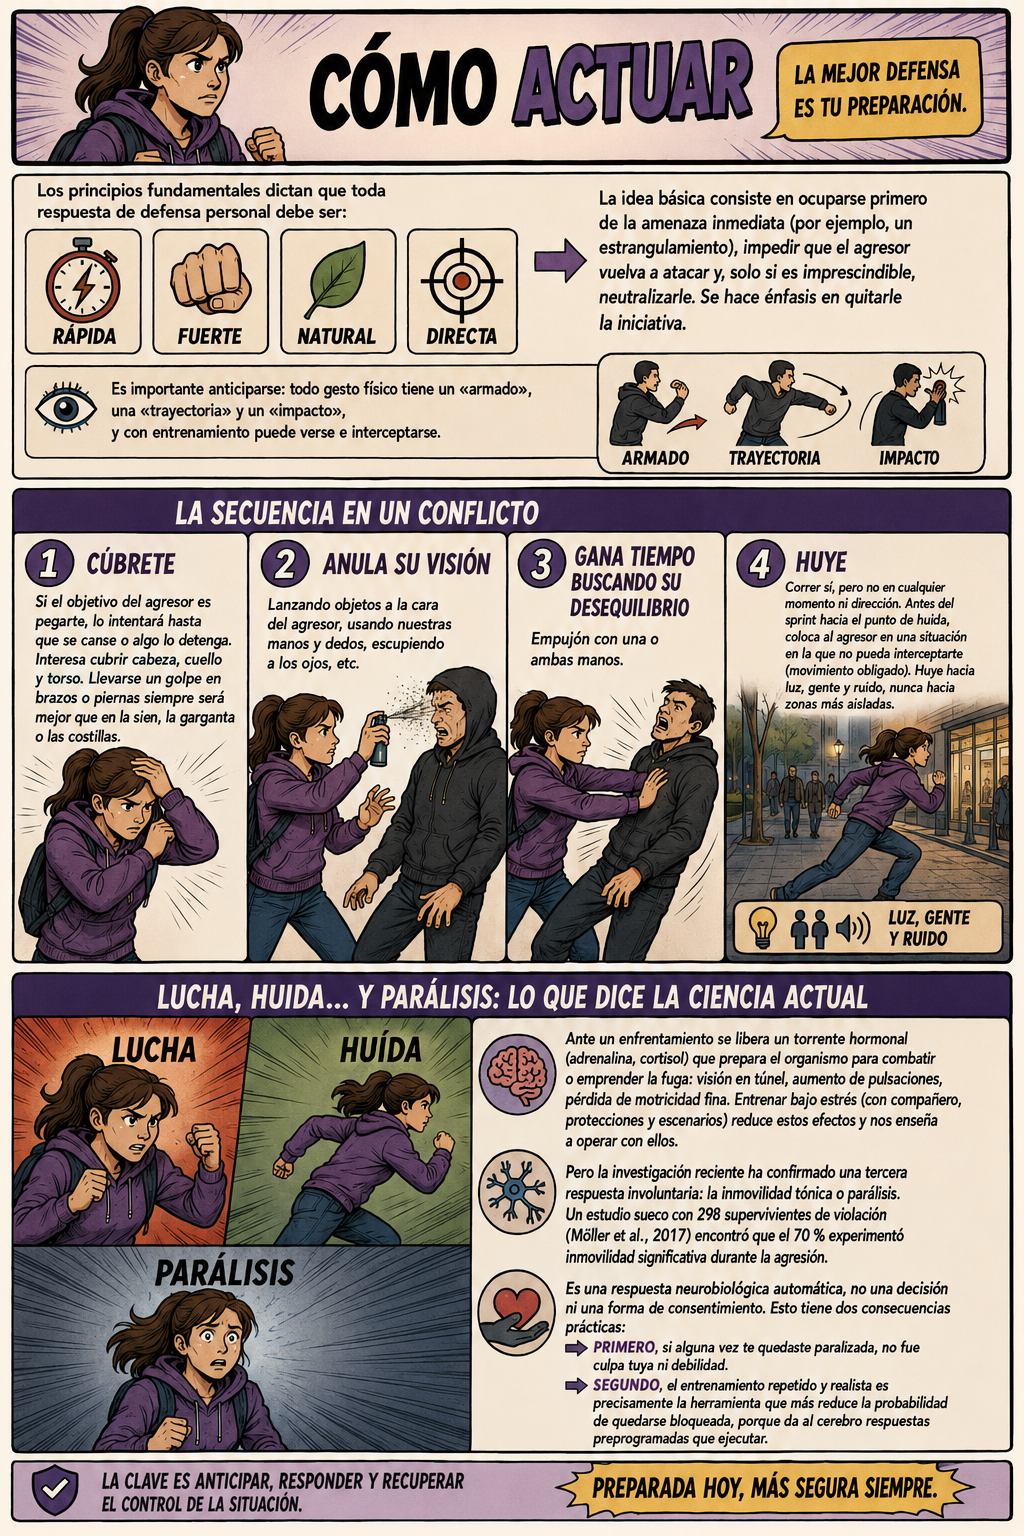
\includegraphics[width=\linewidth]{figures/como-actuar.png}

% =====================================================================
%  Capítulo 5 — Ejercicios de observación
% =====================================================================
\chapter{Ejercicios de observación}
\citacap{Usted ve, pero no observa. La distinción es evidente.}{Sherlock Holmes, en Arthur Conan Doyle}

Permanentemente pasamos por diversos estados de vulnerabilidad: somos más o menos propensas a ser consideradas víctimas. El delincuente común va a elegir al objetivo menos complicado, y va a preferir a quien perciba como menos apta para defenderse por cuestión de edad, salud, distracción o descuido (llevar el bolso colgando a la espalda, el móvil en la mano absorbiendo toda la atención, la mano con reloj en la ventanilla del coche).

\textbf{Primer ejercicio:} dedica unos momentos al andar a ponerte en el rol de alguien que busca una víctima, y estudia a las demás personas para saber a quiénes y por qué \enquote{elegirías}. Observa qué factores transmiten vulnerabilidad y cuáles hacen descartar a otras personas.

\textbf{Segundo ejercicio:} también en la calle, toma consciencia de las personas que te rodean y determina su actividad: si van camino del trabajo o merodean; si algunas están solas pero parecen comunicarse visualmente con otras. Realiza detenciones periódicas ante escaparates y, con una mirada rápida, percibe si alguien hace tu mismo camino.

\textbf{Tercer ejercicio:} al entrar en cualquier local (bar, tienda, vagón), localiza en tres segundos las salidas y a las personas presentes. Al llegar a tu portal o coche, ten las llaves ya en la mano y mira alrededor antes de abrir.

El objetivo no es andar por la calle como una paranoica, sino que, al realizar todo esto a modo de juego, desarrollaremos gradualmente la observación y la capacidad de estar preparadas de forma natural, fijándose estos hábitos sin que nos demos cuenta.

\newpage

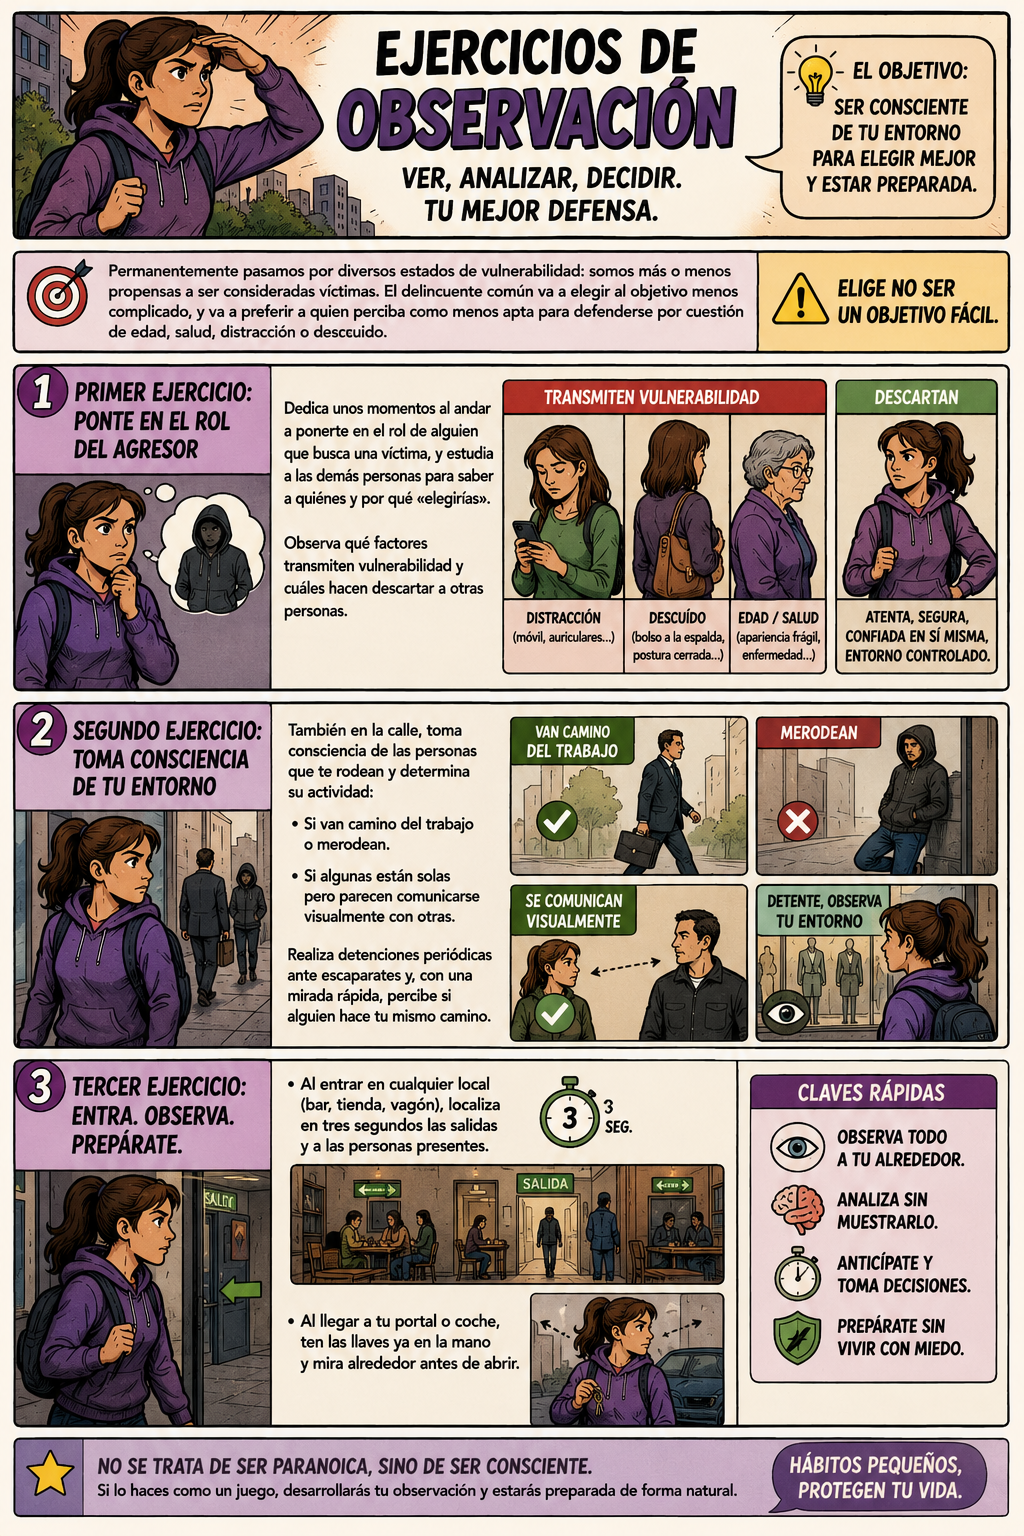
\includegraphics[width=\linewidth]{figures/observacion.png}

% =====================================================================
%  Capítulo 6 — Cuestiones legales
% =====================================================================
\chapter{Cuestiones legales}

Toda agresión puede tener dos tipos principales de consecuencias:

\begin{enumerate}
  \item \textbf{Físicas:} en la salud de la víctima o del agresor (heridas o muerte). Con frecuencia la víctima puede quedar con secuelas psicológicas de largo tratamiento, aun sin sufrir daño físico.
  \item \textbf{Legales:} dado que no pretendemos atacar a nadie, cualquier violencia ejercida sobre quien nos agrede parecería justificada. Sin embargo, para la ley esto no es tan sencillo.
\end{enumerate}

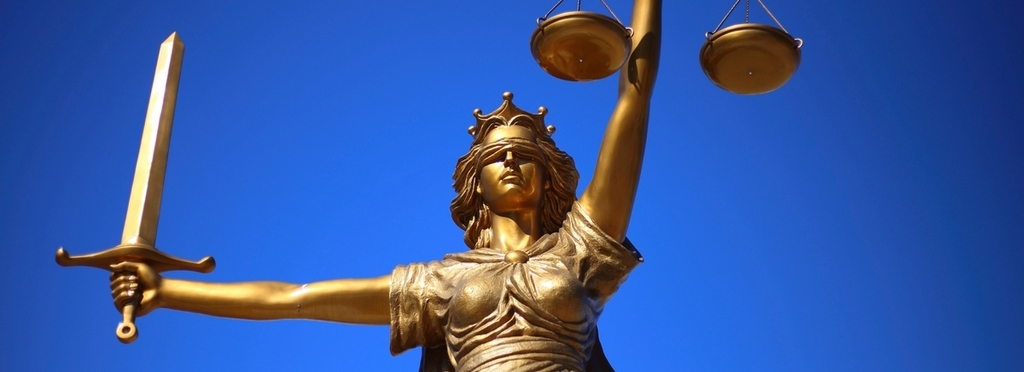
\includegraphics[width=\linewidth]{figures/ley.jpg}

\section{La legítima defensa en España (art.\ 20.4 del Código Penal)}

El Código Penal español \citep{codigopenal1995} exime de responsabilidad criminal a quien obra en defensa de la persona o derechos propios o ajenos, siempre que concurran tres requisitos:

\begin{enumerate}
  \item \textbf{Agresión ilegítima:} un ataque actual o inminente contra ti, otra persona o tus bienes. No vale frente a una agresión ya terminada (entonces sería represalia).
  \item \textbf{Necesidad racional del medio empleado:} la respuesta debe ser razonable para impedir o repeler la agresión, valorando las circunstancias (tamaño y número de agresores, armas, lugar, hora, posibilidad real de huir). No se exige una igualdad matemática de medios: la jurisprudencia reconoce que una mujer frente a un agresor físicamente superior puede necesitar medios más contundentes para defenderse con eficacia.
  \item \textbf{Falta de provocación suficiente:} que quien se defiende no haya provocado la agresión.
\end{enumerate}

El concepto de \enquote{arma} no está reservado a las de fuego y blancas: es todo elemento que aumenta el poder ofensivo de una persona y puede ocasionar lesiones o la muerte. Ten en cuenta, además, que en España está prohibido portar armas e imitaciones en la vía pública (Reglamento de Armas), y que los esprays de defensa solo son legales los homologados por Sanidad para mayores de edad.

Se deben tener en cuenta también las circunstancias: no es lo mismo defenderse de noche de un ladrón que, en pleno día, de un individuo con sus sentidos alterados por alguna droga; la justicia puede valorar su estado, y si causamos daños deberemos poder acreditar que no había otra posibilidad (testigos, cámaras, etc.).

\textbf{Nuestro consejo práctico:} lo primero es salir de la situación de peligro; de las consecuencias nos preocuparemos después. No sabemos cuáles son las intenciones del agresor, así que lo mejor es librarse de él cuanto antes. Solucionemos los problemas según nos vamos encontrando con ellos. La mejor salida de un enfrentamiento sigue siendo evitar el uso de la fuerza, por sus posibles consecuencias: daños físicos o psicológicos, problemas judiciales y posibles venganzas. Y recuerda: no merece la pena sufrir daños por defender un bien material.

\section{Después de una agresión}

\begin{itemize}
  \item Ponte a salvo y llama al \recurso{112} (emergencias) o usa el botón SOS de AlertCops.
  \item Si has sufrido una agresión sexual, acude a urgencias hospitalarias sin lavarte ni cambiarte de ropa, para preservar pruebas; allí se activa el protocolo forense y de atención.
  \item Denuncia en Policía Nacional (\recurso{091}), Guardia Civil (\recurso{062}) o juzgado de guardia. Aporta todos los datos que hayas podido registrar: lugar, número de agresores, edades, armas, estatura, ropa, tatuajes y particularidades.
  \item Las Oficinas de Asistencia a las Víctimas del Delito (Ministerio de Justicia) ofrecen apoyo jurídico y psicológico gratuito.
\end{itemize}

Este capítulo es divulgativo y no constituye asesoramiento jurídico; ante un caso concreto consulta con un abogado.

% =====================================================================
%  Capítulo 7 — Tipos de agresores
% =====================================================================
\chapter{Tipos de agresores}

A continuación presentamos los tipos más comunes de agresores, según sus objetivos y su forma de proceder habitual, para desarrollar una estrategia personal según el caso. Debemos tener en cuenta que pueden presentar trastornos psiquiátricos o estar bajo la influencia de drogas: hay que determinar rápidamente si su condición es de inferioridad física (p.\,ej., alcohol) o lo contrario (p.\,ej., estimulantes), para actuar en consecuencia.

\begin{table}[h]
\centering
\renewcommand{\arraystretch}{1.3}
\small
\begin{tabularx}{\linewidth}{@{}>{\bfseries}l X l l@{}}
\toprule
\textbf{Objetivo} & \textbf{Táctica / Estrategia} & \textbf{Víctimas} & \textbf{Nombre} \\
\midrule
Dinero & Robo, atraco, tirón, secuestro\ldots{} & Hombres y mujeres & Ladrón \\
Ego & Peleas (normalmente sin estrategia, sucediéndose las técnicas) & Más hombres & Buscapeleas \\
Sexo / poder & Abordar por sorpresa o, mucho más a menudo, abusar de una relación de confianza previa & Más mujeres & Agresor sexual \\
Control & Violencia física y psicológica continuada dentro de la pareja o expareja & Mujeres & Maltratador \\
\bottomrule
\end{tabularx}
\end{table}

\section{Ladrón}

El delito más común es el robo con intimidación por armas o por número de delincuentes. Lo primero es establecer cuántos son, ya que podemos ser sorprendidas por cómplices en el momento de realizar una acción defensiva.

Enfrentarse a más de una persona no es aconsejable: se recomienda mantener la calma, entregar los bienes solicitados, no mirar fijamente los rostros (miradas fugaces; los delincuentes temen el reconocimiento) y no provocarles. Es decir, concluir la situación lo antes posible y resultar ilesa, dirigiéndose de inmediato a efectuar la denuncia aportando todos los datos posibles. Ningún objeto vale más que tu integridad.

\section{Buscapeleas}

Ser elegida por este tipo de individuo es un gran problema: generalmente no persigue el robo, sino que se trata de personas guiadas por el deseo de hacer daño (por satisfacción personal, por el público\ldots{}). Están acostumbrados a soportar dolor, tienen un gran repertorio de técnicas sucias y son poco proclives a abandonar mediante el diálogo. Suelen iniciar el ataque con un golpe de improviso.

\begin{itemize}
  \item En estos enfrentamientos no hay reglas: todo vale a efectos de ataque y defensa (como los golpes a genitales), y no se debe mostrar clemencia, porque el atacante no la tendrá.
  \item Busca elementos del entorno (palos, botellas\ldots{}) a modo de arma defensiva, valorando que exhibirlos puede escalar el conflicto si él también tiene acceso a armas o acompañantes. Se pueden usar paredes cercanas o el suelo para empujar contra ellos al rival.
  \item Pon al oponente en el peor terreno: llévalo hacia suelo desfavorable, colócate a un nivel más alto y, de noche, de espaldas a la luz (que le dé en la cara).
  \item Mantén la tranquilidad para no atacar a lo loco, sino a los puntos vulnerables que queden expuestos y con tus técnicas preferidas.
  \item No dudes: provoca una distracción verbal o arrojando algo a la cara, y de inmediato golpea con decisión, combinando manos y pies con técnicas sencillas.
  \item No te confíes: ni de las palabras ni de una aparente rendición; no des nunca la espalda ni relajes la atención.
  \item Termina lo más rápido posible y retírate del lugar de inmediato.
\end{itemize}

Estadísticamente, según el género del agresor su forma de actuar es distinta. Si es hombre, lo habitual son golpes a puño cerrado, golpes ascendentes si la agredida se inclina, abrazos al cuerpo y cuello, patadas frontales a genitales o circulares al pecho y cabeza, y cabezazos en la corta distancia. Si es mujer, lo habitual son golpes a mano abierta y arañazos, estirones al suelo, agarres al pelo, cuerpo y cuello, pisotones y patadas descendentes, y escupitajos en la corta distancia.

\newpage

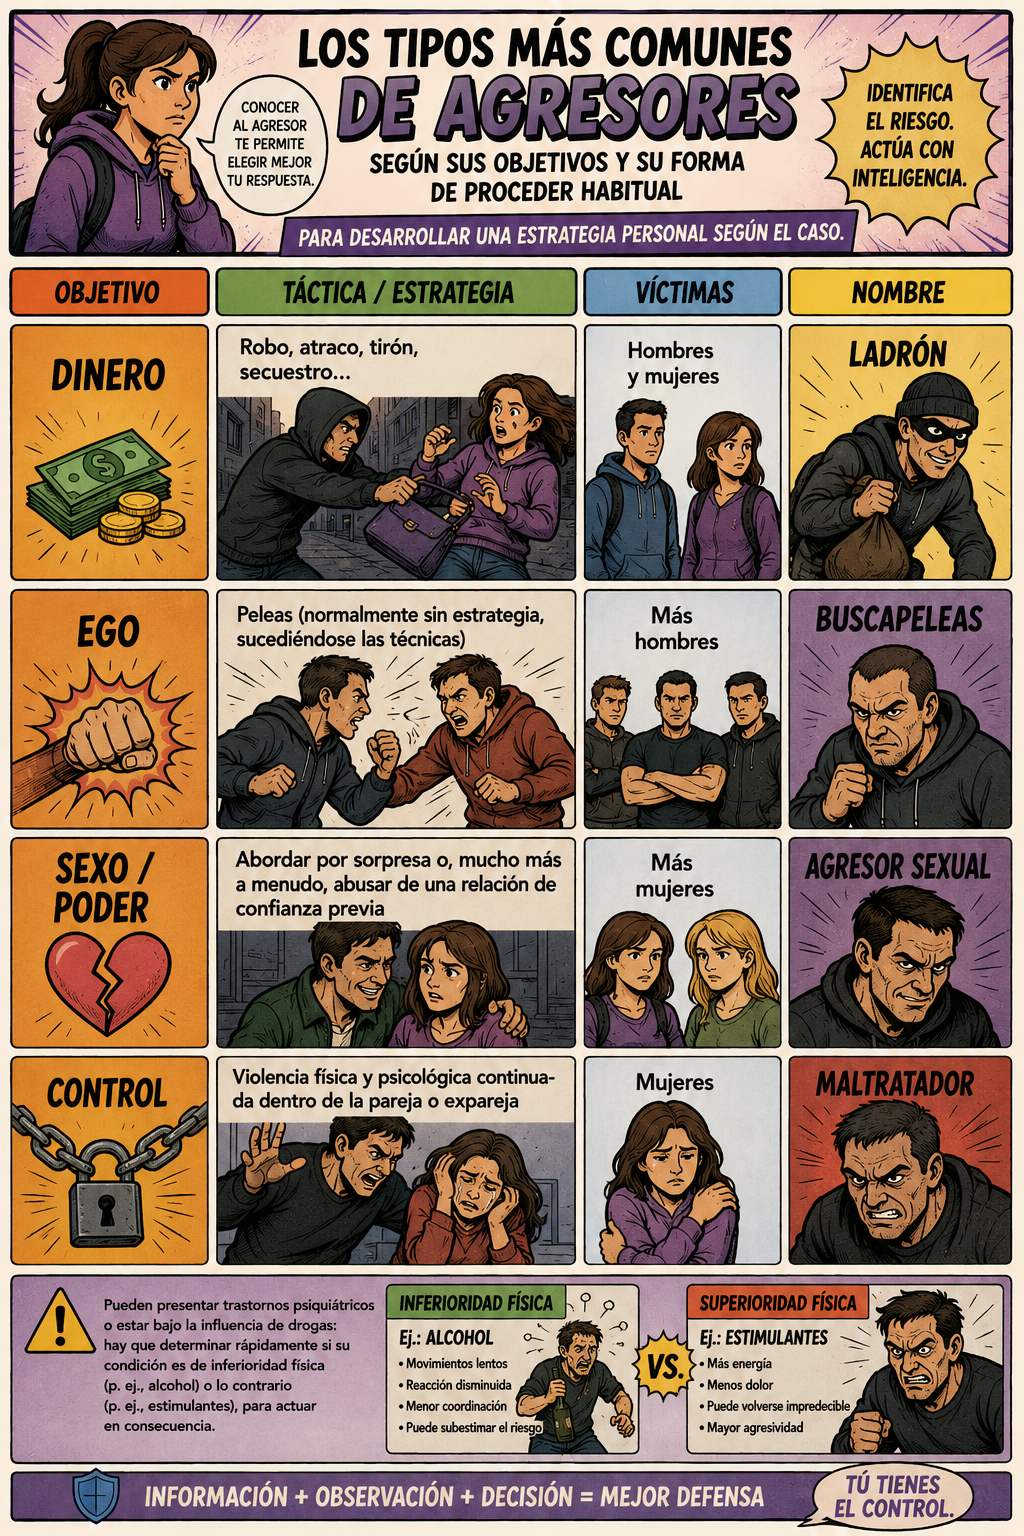
\includegraphics[width=\linewidth]{figures/agresores.png}
% =====================================================================
%  Capítulo 8 — El agresor sexual: prevención y respuesta
% =====================================================================
\chapter{El agresor sexual: prevención y respuesta}

Para enfrentarse a un agresor sexual es aplicable todo lo visto en los puntos precedentes, pero hay que mencionar variables propias de este tipo de agresiones. La primera y más importante, confirmada por todas las estadísticas (incluida la Macroencuesta de Violencia contra la Mujer del Ministerio de Igualdad): en la gran mayoría de los casos el agresor NO es un extraño, sino alguien del entorno: pareja o expareja, conocidos, compañeros de trabajo o estudios. El estereotipo del desconocido en el callejón existe, pero es minoritario.

\section{Prevención}

\begin{itemize}
  \item Es posible cortar muchas situaciones poniendo límites enérgicos en la etapa previa, cuando se hace evidente la presión psicológica: nombrar la conducta (\enquote{esto es acoso}), exigir que cese y, si procede, amenazar con denuncia delante de testigos. El acosador cuenta con el silencio.
  \item Evita compartir lugares de riesgo con un potencial agresor: ascensores, \enquote{entrevistas de trabajo} fuera de la oficina y del horario laboral, quedadas a solas con desconocidos sin que nadie sepa dónde estás. Este tipo de ataques solo se realizan en lugares seguros para el atacante: niégale ese terreno.
  \item No des información personal (teléfono, dirección, rutinas) a cualquier compañero o jefe solo por agradar.
  \item En citas con personas conocidas por internet: primer encuentro en lugar público, avisa a alguien de confianza (o usa la función Guardián/Acompáñame de AlertCops), vigila tu bebida y ten transporte de vuelta propio.
  \item La sumisión química existe: no aceptes bebidas que no hayas visto servir y no dejes tu vaso sin vigilancia. Si notas mareo o confusión desproporcionados, pide ayuda inmediatamente a personal del local o amigas.
\end{itemize}

\section{Si el ataque llega: qué dice la evidencia}

Durante décadas se aconsejó de forma genérica \enquote{no resistirse}. La investigación actual lo matiza de forma importante: los estudios sobre resistencia \citep{ullman1997, ullman2007, tark2014} muestran que la resistencia activa ---gritar, forcejear, golpear, huir--- reduce significativamente la probabilidad de que la violación se consume, y que en la mayoría de los casos no incrementa las lesiones físicas adicionales: la lesión suele preceder a la resistencia, no ser su consecuencia. Por eso los programas modernos de autodefensa femenina entrenan la resistencia verbal y física inmediata y decidida.

Dicho esto, ninguna estadística decide por ti en el momento: cada situación es única (armas, encierro, varios agresores) y TODA estrategia de supervivencia es legítima, incluida la sumisión táctica para ganar tiempo y esperar una oportunidad. Quien sobrevive, lo hizo bien. La culpa es siempre del agresor.

\section{La oportunidad y la sorpresa}

Comúnmente los agresores sexuales no tienen especial experiencia en combate, por lo que una persona decidida puede causar un gran daño en un individuo ocupado en otros menesteres que no son la pelea. El agresor suele subestimar a la mujer porque la supone débil: si aparentas rendición, bajará su atención defensiva, y ese es el momento de actuar con total decisión. El riesgo psicológico a evitar es ponerse mentalmente en un plano de inferioridad que anule la acción: contra eso se entrena.

Una vez lograda la oportunidad, se imponen procedimientos que deben repasarse mentalmente y que, aunque parezcan excesivos, son proporcionados frente a una violación:

\begin{itemize}
  \item Con la cara del agresor cerca, hundir fuerte y profundamente los pulgares en los ojos.
  \item Empuñar elementos del entorno: en una oficina, un bolígrafo (asegurando la parte trasera con el pulgar) contra las partes blandas.
  \item La mandíbula desarrolla una potencia enorme: usar la boca para morder y desgarrar partes blandas de cara y cuello.
  \item Combinar todo con golpes contundentes de codo o estrellando la cabeza del agresor contra elementos duros, gritar para alertar, y retirarse rápidamente para pedir ayuda y denunciar.
\end{itemize}

Nunca sabemos las intenciones finales del agresor, así que no hay que tener ningún reparo ni compasión a la hora de defenderse.

\section{Si un asaltante te agarra, recuerda}

\begin{itemize}
  \item Si te agarra bien, será mucho más difícil escapar: actúa pronto.
  \item Si sus manos están ocupadas agarrándote, otros objetivos (ojos, garganta, genitales) se presentan por sí mismos.
  \item Muévete: hay que ser escurridiza.
  \item Grita órdenes concretas: \enquote{¡Suéltame!}, \enquote{¡Fuego!}, \enquote{¡Llamad a la policía!}. El grito te activa, te hace respirar, desconcierta y atrae testigos.
\end{itemize}

Si intentas una técnica para escapar y no funciona, no te rindas: intenta otra. Haz lo inesperado. Trabajar con un instructor que lleva protecciones te dará una idea de cómo se siente realmente intentar liberarse.

% =====================================================================
%  Capítulo 9 — Violencia en la pareja: el agresor conocido
% =====================================================================
\chapter{Violencia en la pareja: el agresor conocido}

Un manual de defensa personal para mujeres quedaría incompleto sin abordar el escenario estadísticamente más probable: la violencia ejercida por la pareja o expareja. Aquí la \enquote{distancia preventiva} no es física sino temporal: detectar las señales cuanto antes.

\section{Señales de alarma tempranas}

\begin{itemize}
  \item Control: del móvil, la ropa, el dinero, las amistades, la ubicación.
  \item Aislamiento progresivo de familia y amigas.
  \item Celos presentados como \enquote{amor}; vigilancia de redes sociales.
  \item Humillaciones, desprecio a tus opiniones, cambios bruscos de humor.
  \item Empujones, golpes a objetos, amenazas\ldots{} seguidos de arrepentimiento y \enquote{luna de miel}. El ciclo de la violencia (tensión -- explosión -- arrepentimiento) tiende a acortarse y agravarse con el tiempo.
\end{itemize}

\section{Plan de seguridad}

\begin{itemize}
  \item Memoriza los teléfonos clave (\recurso{016}, \recurso{112}) y mantén el móvil cargado y contigo.
  \item Instala AlertCops y activa el Botón SOS (ver capítulo de aplicaciones): pulsándolo 5 veces en menos de 6 segundos envía alerta y audio a la policía.
  \item Prepara una bolsa de emergencia (documentación, llaves, dinero, medicación) en casa de alguien de confianza.
  \item Acuerda una palabra clave con familiares o vecinas que signifique \enquote{llama a la policía}.
  \item Identifica las zonas seguras de la casa (con salida, sin objetos peligrosos: evita cocina y baño durante las explosiones).
  \item Guarda pruebas: partes médicos, mensajes, fotografías de lesiones.
\end{itemize}

\section{Recursos específicos en España}

\begin{itemize}
  \item \recurso{016:} teléfono gratuito y confidencial, 24 horas, en varios idiomas. No deja rastro en la factura (recuerda borrarlo del registro de llamadas). También WhatsApp \recurso{600 000 016} y correo \href{mailto:016-online@igualdad.gob.es}{016-online@igualdad.gob.es}.
  \item \recurso{ATENPRO:} servicio telefónico de atención y protección con terminal móvil y localización, para víctimas con orden de protección (se solicita en servicios sociales).
  \item \recurso{Sistema VioGén:} seguimiento policial integral de los casos denunciados.
  \item \recurso{En emergencia:} \recurso{112}, \recurso{091} (Policía Nacional), \recurso{062} (Guardia Civil) o botón SOS de AlertCops.
\end{itemize}

% =====================================================================
%  Capítulo 10 — Tipos de agresiones
% =====================================================================
\chapter{Tipos de agresiones}
\citacap{Quien conoce el peligro aprende a evitarlo.}{Proverbio}

El agresor puede interactuar con nosotras de las siguientes formas:

\begin{enumerate}
  \item Golpes con la mano dominante (diestra o zurda), con o sin agarre de la otra.
  \item Golpes con ambas manos: alternos o aleatorios.
  \item Golpes que no llegan a impactar, en muchas ocasiones desequilibrando al agresor (por buen movimiento de la agredida o error de cálculo del agresor).
  \item Golpes que impactan, llevando a doblegarse o caer al suelo.
  \item Agarres, con tres posibilidades: \textbf{(a)} agarre que busca trasladarme a un sitio donde no quiero ir ---de un agarre pasará a otro hasta cambiar la dinámica---; \textbf{(b)} agarre que busca que me quede estática, muchas veces golpeando con la otra mano; \textbf{(c)} agarre intimidatorio, para recortar distancia y amenazar con superioridad física.
\end{enumerate}

\begin{reglaoro}
\textbf{Contra el traslado:} nunca dejarse llevar a un \enquote{segundo lugar} (un coche, un portal, un descampado). Las estadísticas policiales coinciden: el segundo lugar siempre es peor que el primero, porque es el terreno elegido por el agresor. Resiste, grita y lucha en el primer escenario, donde aún hay testigos posibles.
\end{reglaoro}

\newpage

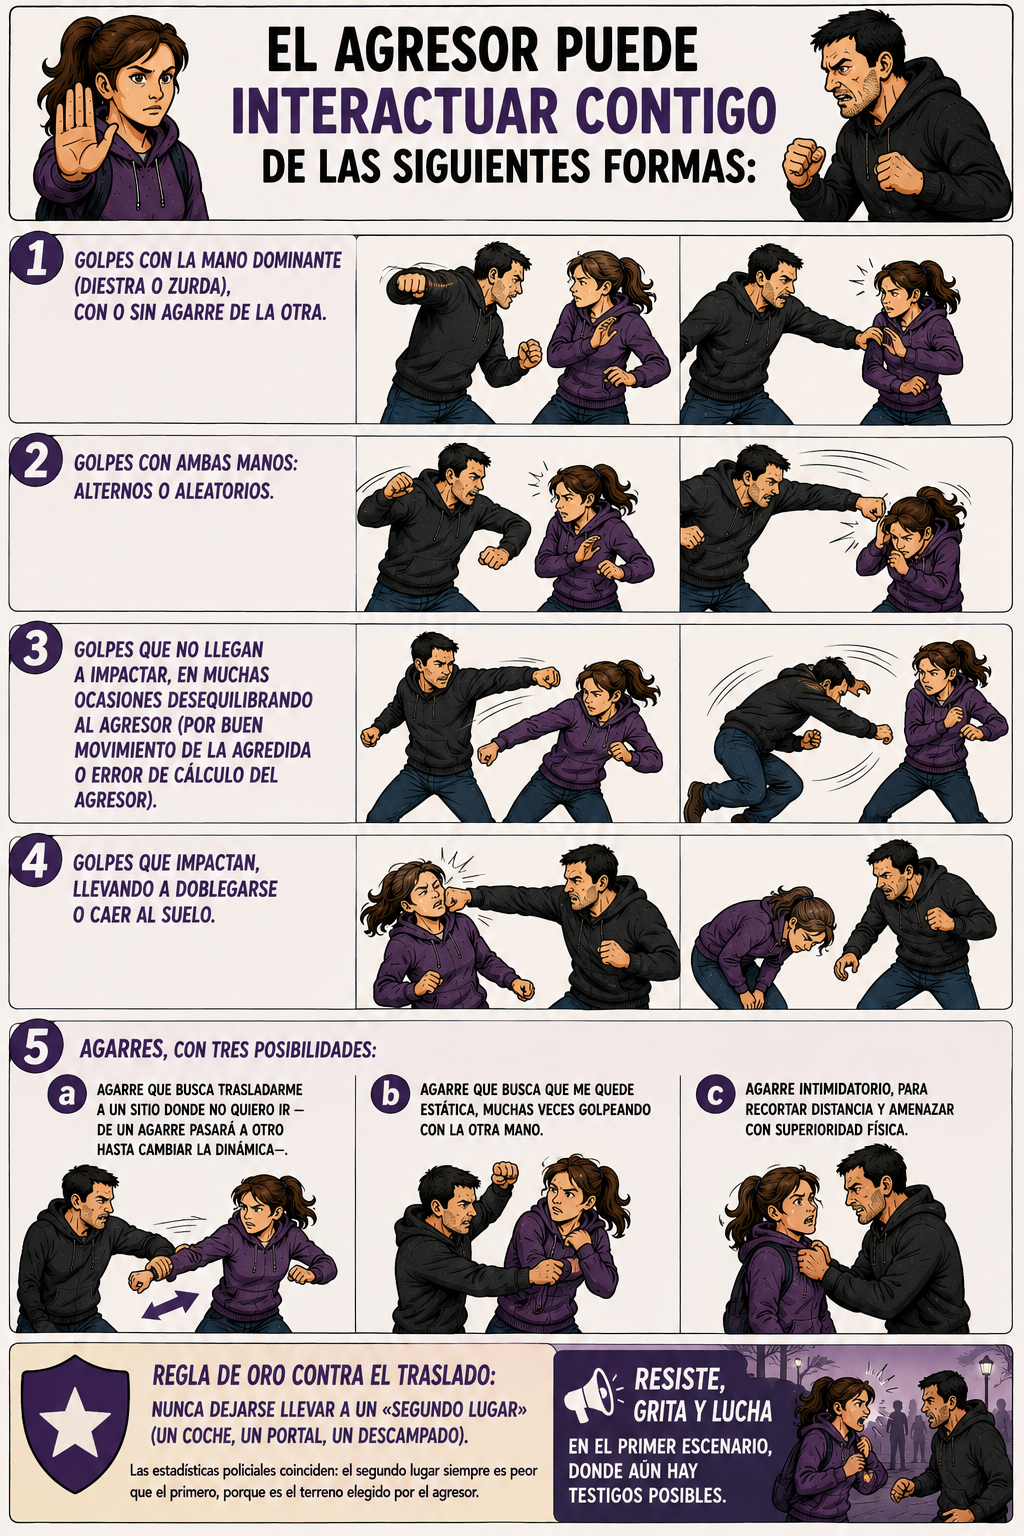
\includegraphics[width=\linewidth]{figures/tipos-agresiones.png}
% =====================================================================
%  Capítulo 11 — Entrenamiento
% =====================================================================
\chapter{Entrenamiento}

La preparación psicológica es la más importante: las cualidades físicas de nada sirven cuando no son controlables debido a las emociones intensas por la descarga de adrenalina (visión en túnel, aumento de latidos, rigidez muscular). Pero también es cierto que cuanto mejor sea el estado de nuestro cuerpo, más posibilidades habrá de salir bien librada.

Por ello se iniciará el entrenamiento básico de las armas corporales, descartando movimientos rebuscados y aprovechando la natural potencia de algunas zonas. Primaremos el uso de golpes, que pueden entrenarse en el aire (cosa no muy recomendable) pero que se dominan con un mínimo de equipo: manoplas, saco, o incluso un saco de dormir sujetado por alguien.

\begin{itemize}
  \item La efectividad no se consigue solamente con el conocimiento, sino con la práctica.
  \item La práctica ha de ser progresiva: primero lentamente, cuidando la forma correcta sin forzar el organismo; después incrementando velocidad y potencia.
  \item No golpeamos reteniendo la respiración ni inspirando, sino exhalando para acompañar el golpe.
  \item Antes de entrenar con fuerza, calienta el organismo unos quince minutos.
  \item Visualiza: imagina que estás frente a un adversario y en qué parte de su cuerpo golpeas.
  \item Si es posible, entrena con compañero y equipos protectores para acostumbrarte a la sensación de ser agredida, e incluye escenarios con voz: marcar límites gritando antes del contacto.
\end{itemize}

% =====================================================================
%  Capítulo 12 — Puntos a golpear
% =====================================================================
\chapter{Puntos a golpear}

El daño producido por un golpe en partes específicas donde el organismo es más vulnerable es mucho mayor que en cualquier otro punto al azar. Estos puntos se denominan \enquote{puntos vitales}, no porque su ataque determine la muerte instantánea, sino porque el efecto es muy superior al de las zonas vecinas. Lograr un golpe definitivo es bastante difícil: dependen de la resistencia corporal, la potencia, la técnica, el equilibrio y el movimiento. Recuerda el marco legal: estos recursos se justifican por la necesidad racional de interrumpir una agresión, no para prolongarla.

Estas regiones pueden atacarse con golpes o con presiones de dedos. Es recomendable familiarizarse con ellas presionando suavemente en el propio cuerpo hasta ubicar el lugar exacto de sensibilidad. Intentaremos golpear: espacios intermusculares y sistema nervioso periférico, arterias y venas, órganos huecos, articulaciones, músculos y huesos.

\section{Los puntos más accesibles con técnicas simples}

\begin{itemize}
  \item \textbf{Ojos:} muy sensibles; pueden atacarse con la punta de los dedos y objetos punzantes, presionarse contra el borde orbitario, o usarse para distracciones (arrojar tierra, llaves o un simple amago) que regalan el segundo necesario para atacar o huir.
  \item \textbf{Entrecejo:} aloja el hueso etmoides, esponja ósea muy vascularizada; su fractura (con elementos contundentes) provoca gran hemorragia. La frente, en cambio, es de las zonas más duras: golpearla con el puño puede fracturarnos la mano.
  \item \textbf{Nariz:} su fractura provoca dolor y lagrimeo; el golpe con la base de la palma es seguro para nuestra mano.
  \item \textbf{Boca:} su rotura es muy invalidante, pero no debe atacarse con la mano desnuda (riesgo de heridas e infección por mordedura), sino con objetos o con el codo.
  \item \textbf{Oídos:} sensibles al impacto con la palma abierta (\enquote{sopapo} que aumenta la presión y lesiona el tímpano).
  \item \textbf{Laringe y garganta:} muy susceptible a golpes; atacarla puede provocar desmayo e incluso la muerte: reservar para peligro extremo.
  \item \textbf{Clavículas:} se buscan fracturas con golpes tipo \enquote{martillo} del puño o con elementos contundentes para incapacitar el brazo.
  \item \textbf{Dedos de las manos:} clave para romper agarres (hasta del pelo): toma cualquier dedo y haz palanca para hiperextenderlo.
  \item \textbf{Manubrio del esternón:} metiendo un dedo en el hueco sobre el esternón y empujando hacia atrás y abajo se gana distancia (probar suavemente en el propio cuerpo).
  \item \textbf{Plexo solar:} golpearlo afecta a la red nerviosa abdominal y provoca incapacitación temporal.
  \item \textbf{Genitales:} efecto similar al anterior; se atacan con patada en distancia larga, rodillazo en la corta o agarre/apretón en el cuerpo a cuerpo.
  \item \textbf{Rodilla:} se ataca con patadas (punta o tacón del zapato sobre la rótula) para reducir la movilidad. Los golpes bajos son rápidos, difíciles de detener y crean sorpresa para enlazar otra técnica.
  \item \textbf{Tibia:} patear de frente su cara interna (sin musculatura) provoca dolor agudo; de espaldas, con el talón, sirve contra agarres por detrás.
  \item \textbf{Empeine y dedos de los pies:} pisotones de frente o con el tacón hacia atrás para liberarse de agarres; su fractura puede definir un enfrentamiento al impedir la movilidad.
\end{itemize}

\newpage

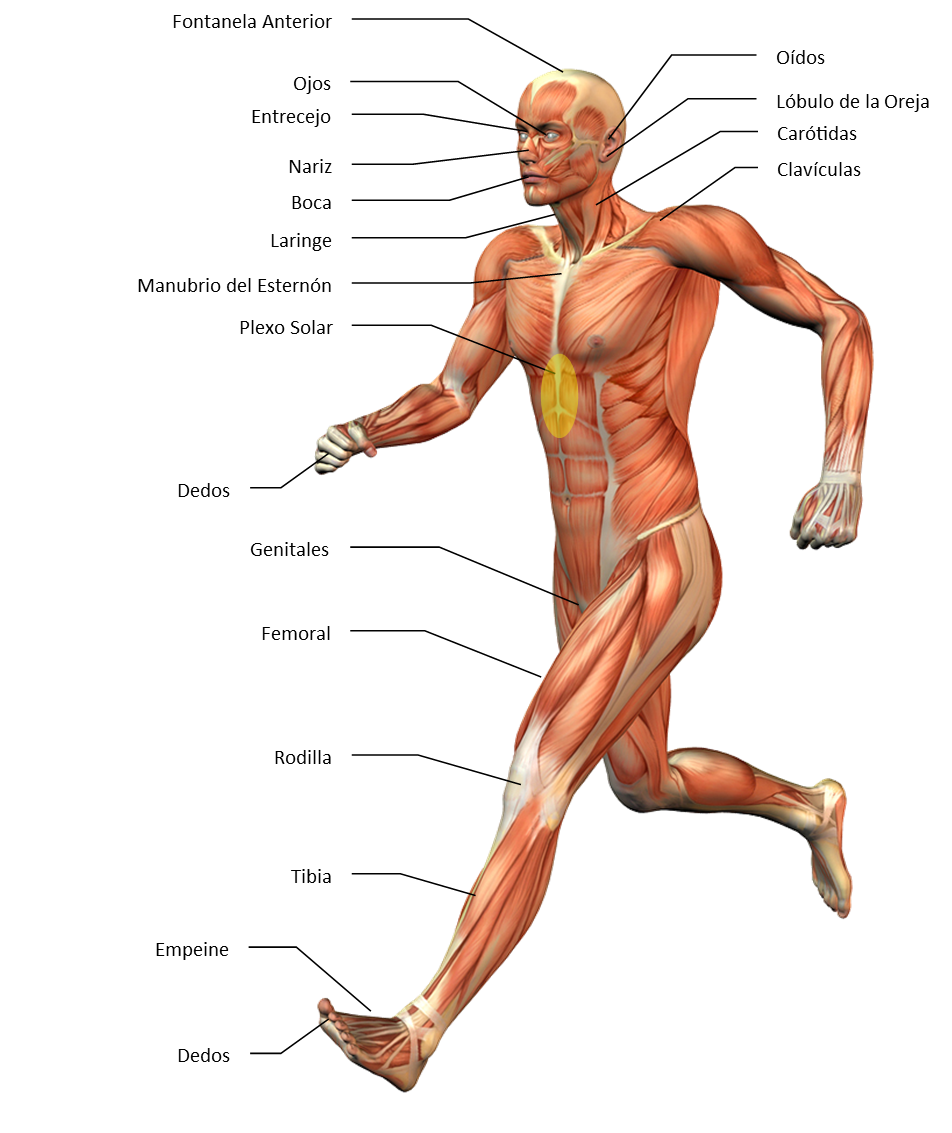
\includegraphics[width=\linewidth]{figures/Imagen8.png}

% =====================================================================
%  Capítulo 13 — Guardia y distancia
% =====================================================================
\chapter{Guardia y distancia}

Antes de ejecutar un golpe es importante estar equilibrada: columna estirada, con el peso de la parte superior dentro de la base que forman las piernas. Postura relajada, peso repartido entre los dos pies separados aproximadamente la anchura de los hombros, uno adelantado apuntando al frente y el otro atrasado a 45 grados hacia fuera. Con el peso sobre las puntas de los pies (asentarse en los talones desequilibra), flexionamos rodillas y ajustamos el tórax hasta movernos sin tambalearnos.

Es importante practicar esto hasta adoptar la posición instintivamente ante un peligro. Aunque la posición de los brazos en la calle no ha de ser agresiva, sí ha de estar atenta a bloquear: una \enquote{guardia de paz} con las palmas abiertas a la altura del pecho, en gesto de calma (\enquote{tranquilo, no quiero problemas}), protege sin provocar y deja las manos listas. Para entrenar dispondremos una guardia de mano abierta similar a la de los boxeadores, con el brazo no dominante adelante: el brazo adelantado protege desde la boca hasta el abdomen y el atrasado está listo para lanzar el ataque.

De pie frente a un compañero, medimos la distancia a la que debemos estar para llegar de manera efectiva con nuestras diferentes armas corporales. Cada persona tiene una distancia diferente según su anatomía, y debemos acostumbrarnos a no lanzar golpes que no van a impactar:

\begin{itemize}
  \item Distancia larga: patadas.
  \item Distancia media: manos.
  \item Distancia corta: codos y rodillas.
  \item Cuerpo a cuerpo.
\end{itemize}

En defensa personal entrenaremos sobre todo la distancia media, corta y el cuerpo a cuerpo, dejando las patadas altas a las artes marciales (requieren práctica habitual y comprometen el equilibrio). Hasta acostumbrarnos a golpear, atención a no estirar los miembros por completo: deben quedar imperceptiblemente retraídos para no dañar las articulaciones con cada golpe.

\section{Golpes de distancia media: la mano}

Si no tenemos entrenamiento en deportes de contacto, golpearemos con la mano abierta, utilizando la palma y su base (dedos semiextendidos y apretados): es más segura para nuestros huesos que el puño. Partiendo de la guardia, proyectamos la mano hacia la cabeza del oponente en un movimiento circular, teniendo en cuenta:

\begin{itemize}
  \item Acompañar cada golpe con la exhalación del aire.
  \item Corregir la distancia: ni tan corta que apenas toque, ni tan larga que el brazo no tenga recorrido.
  \item Comenzar sin potencia ni velocidad hasta familiarizarse con la técnica; después incrementar siempre dentro de la comodidad y sin dolor.
\end{itemize}

Cada golpe debe realizarse en equilibrio, pies bien asentados, acompañando cada mano con su giro de cadera. Por último, se practicarán estos golpes desde una actitud no agresiva (posición de descanso o \enquote{guardia de paz}) y de forma sorpresiva, sin movimientos previos que delaten la intención.

\section{Golpes de distancia corta: el codo}

El codo posee potencia y dureza naturales aun en personas que nunca han practicado artes de combate. Partimos de la guardia a distancia corta. Como con la mano, son primordiales el equilibrio y el giro de cadera: siempre será más fuerte el codazo de la pierna retrasada, al contar con mayor trayectoria. Proyectamos el codo hacia delante paralelo al suelo (el puño termina horizontal delante del pecho) impactando con la zona vecina a la punta.

Tras el golpe, la cintura queda colocada para sacar el otro codo girando la cadera en sentido opuesto, encadenando codazos. Con entrenamiento percibiremos esta mecánica y su progresiva potencia. Se sugiere su uso a muy corta distancia y para sorprender con un fuerte golpe a la mandíbula que provocará la confusión suficiente para seguir encadenando. Dominado el golpe horizontal, conviene entrenarlo en otras direcciones: ascendente a la mandíbula, descendente, y hacia atrás contra agarres por la espalda. Los codos también son muy recomendables para interponerse en la trayectoria de golpes y patadas.

\section{Golpes de distancia corta: la rodilla y golpes bajos}

La rodilla es un arma fuerte y dura por naturaleza: impactaremos en el ángulo que nos sea cómodo (ascendente al frente, o circular de fuera a dentro en corta distancia). Tendrá más efecto el rodillazo de la pierna atrasada por la mayor acción de la cadera. Objetivos: genitales y piernas y, según nuestra flexibilidad y la altura del oponente (por ejemplo, si le hemos bajado la cabeza tirando del pelo), estómago, costillas y cara.

Otras técnicas de nivel bajo se inician elevando poco la rodilla, sin anunciar el ataque, y estirando rápidamente la pierna:

\begin{itemize}
  \item Puntapié con la punta del zapato a tibia y rótula.
  \item Patada con la cara interna o externa del pie a tibia y rodilla, en trayectoria recta, como \enquote{cortando} la pierna.
  \item Pisotón al empeine y dedos del pie.
  \item Talonazo hacia atrás, para aflojar agarres desde la espalda.
\end{itemize}

Este entrenamiento, unido al uso de tacones, puede provocar daños de gran consideración por su capacidad de penetración, sobre todo \enquote{clavando} el tacón hacia delante o en pisotón.

\section{Sueltas básicas de agarres}

\begin{itemize}
  \item \textbf{Agarre de muñeca:} gira tu brazo y tira con fuerza hacia el hueco entre su pulgar y sus dedos (el punto débil de todo agarre), acompañando con todo el cuerpo, no solo el brazo.
  \item \textbf{Agarre de pelo:} fija sus manos contra tu cabeza con tus dos manos (quita el dolor y el control), gira hacia él y contraataca a ojos o garganta.
  \item \textbf{Abrazo de oso por detrás:} baja el centro de gravedad, talonazo a empeine/tibia, cabezazo hacia atrás si te aprisiona los brazos, y palanca a un dedo en cuanto liberes una mano.
  \item \textbf{Estrangulamiento frontal:} protege la vía aérea metiendo la barbilla, agarra y desgarra uno de sus meñiques mientras atacas a los ojos; gira el cuerpo para deshacer la presión.
\end{itemize}

Estas descripciones son solo recordatorios para quien las haya practicado: las sueltas requieren práctica supervisada con compañero.

% =====================================================================
%  Capítulo 14 — Aplicaciones móviles de seguridad
% =====================================================================
\chapter{Aplicaciones móviles de seguridad}
\citacap{La tecnología debe ser un aliado de tu atención, nunca un sustituto de ella.}{Anónimo}

El teléfono móvil es hoy una herramienta de autoprotección de primer orden: permite pedir ayuda, compartir ubicación en tiempo real y documentar incidentes. Estas son las aplicaciones recomendadas en España (todas gratuitas y oficiales):

\section{AlertCops (Ministerio del Interior) --- la imprescindible}

AlertCops es la aplicación oficial de seguridad ciudadana de la Secretaría de Estado de Seguridad (Ministerio del Interior), disponible en toda España. Proporciona un canal directo con Policía Nacional y Guardia Civil, con geolocalización de la alerta para que acuda la patrulla más próxima. Sus funciones principales:

\begin{itemize}
  \item \textbf{Alertas con chat:} comunicar cualquier hecho del que seas víctima o testigo, adjuntando fotos, vídeos, audios o tu localización, con respuesta inmediata.
  \item \textbf{Botón SOS:} con protección reforzada para colectivos vulnerables (entre ellos, víctimas de violencia de género). Pulsándolo repetidamente (cinco veces en menos de seis segundos) envía una alerta urgente al centro policial más cercano con tu posición y una grabación de audio de 10 segundos para que los agentes valoren la gravedad.
  \item \textbf{Guardián:} comparte tu ubicación en tiempo real con contactos de confianza o con las Fuerzas de Seguridad.
  \item \textbf{Acompáñame:} para trayectos en los que quieras sentirte acompañada (volver a casa de noche, una cita con un desconocido).
  \item \textbf{Llamada simulada:} genera una llamada falsa que te da excusa para salir de una situación incómoda.
  \item \textbf{Traductor automático} para comunicarse con la policía en más de cien idiomas, y alertas de seguridad y emergencia de tu zona.
\end{itemize}

Descarga oficial (comprueba que el desarrollador es \enquote{Secretaría de Estado de Seguridad - Ministerio del Interior}):

\begin{itemize}
  \item iOS (App Store): \url{https://apps.apple.com/es/app/alertcops/id1273718252}
  \item Android (Google Play): \url{https://play.google.com/store/apps/details?id=com.alertcops4.app}
  \item Web oficial: \url{https://alertcops.ses.mir.es}
\end{itemize}

Tras descargarla, regístrate con tu nombre y número de móvil (validación por SMS) y configura el Botón SOS y tus contactos guardianes ANTES de necesitarlos.

\section{Otras aplicaciones y servicios útiles}

\begin{itemize}
  \item \textbf{My112 / apps oficiales 112 autonómicas:} al llamar a emergencias envían tu posición exacta al centro de coordinación, crucial si no sabes dónde estás. Busca la app 112 oficial de tu comunidad autónoma en las tiendas oficiales.
  \item \textbf{016 Online:} además del teléfono 016, el servicio estatal contra la violencia de género atiende por WhatsApp (\recurso{600 000 016}) y correo (\href{mailto:016-online@igualdad.gob.es}{016-online@igualdad.gob.es}), útil cuando hablar en voz alta es peligroso.
  \item \textbf{Compartir ubicación del propio sistema:} tanto iOS (Buscar/Find My) como Android (Google Maps -- Compartir ubicación) permiten que personas de confianza sigan tu trayecto en tiempo real sin instalar nada más.
  \item \textbf{Función de emergencia del teléfono:} aprende el gesto SOS de tu modelo (en muchos Android e iPhone, pulsar 5 veces el botón lateral llama a emergencias y avisa a tus contactos). Configúralo hoy.
\end{itemize}

\begin{consejo}
\textbf{Consejo:} ninguna app sustituye a la atención al entorno. El móvil en la mano mirando la pantalla te pone en \enquote{código blanco}; el móvil configurado en el bolsillo, con SOS y Guardián listos, es un arma defensiva.
\end{consejo}

% =====================================================================
%  Capítulo 15 — Conclusiones
% =====================================================================
\chapter{Conclusiones}
\citacap{La mejor protección que puede tener una mujer es el valor.}{Elizabeth Cady Stanton}

Llegadas a este punto, ya deberíamos tener una idea de:

\begin{itemize}
  \item En qué circunstancias es oportuno defenderse de otra persona y cuál es el marco legal.
  \item Nuestras propias capacidades para ejecutar unas técnicas, descartar otras o entrenarlas más a fondo.
  \item Mediante la práctica, haber seleccionado movimientos preferidos para cada distancia de conflicto.
  \item Que los ataques deben efectuarse en combinación de técnicas, en series encadenadas y, a ser posible, a diferentes alturas.
  \item Que es de suma importancia la confianza en una misma: la duda genera un ataque débil que probablemente pondrá más violento al agresor. Tomada una decisión, no echarse atrás.
  \item Que se van a experimentar sensaciones corporales poco usuales, y que en situación real se realizan menos golpes, pero más contundentes.
  \item Que debemos estar preparadas mentalmente para recibir golpes o sufrir heridas, sabiendo que el organismo estará en un estado de mayor rendimiento y resistencia al dolor.
  \item Que el torrente hormonal del enfrentamiento es el cuerpo en su máximo punto de rendimiento; y que si alguna vez aparece la parálisis, es una respuesta automática que el entrenamiento ayuda a superar, nunca una culpa.
\end{itemize}

La defensa personal puede perfeccionarse día a día con la observación, la práctica física y el estudio. Lo más importante es la prevención y, llegado el enfrentamiento, la sorpresa (fingirse colaborativa o temerosa y no exteriorizar el ataque que se está por llevar a cabo). Y por último: no merece la pena sufrir daños por defender un bien material.

\section{Teléfonos y recursos esenciales (España)}

\begin{table}[h]
\centering
\renewcommand{\arraystretch}{1.4}
\begin{tabularx}{\linewidth}{@{}>{\bfseries\color{primario}}l X@{}}
\toprule
\textbf{112} & Emergencias generales (UE) \\
\textbf{091} & Policía Nacional \\
\textbf{062} & Guardia Civil \\
\textbf{016 / WhatsApp 600 000 016} & Violencia contra la mujer: gratuito, 24\,h, confidencial, no aparece en factura \\
\textbf{AlertCops (app)} & Chat y botón SOS con Policía y Guardia Civil \\
\textbf{Oficinas de Asistencia a las Víctimas} & Apoyo jurídico y psicológico gratuito (Ministerio de Justicia) \\
\bottomrule
\end{tabularx}
\end{table}


% ====================================================
% MATERIAL FINAL
% ====================================================

\backmatter

\cleardoublepage

% =====================================================================
%  Material posterior — Fuentes, bibliografía y licencia
%  La lista de referencias se genera con BibTeX a partir de
%  bibliography/referencias.bib (estilo autor-año, natbib + plainnat).
% =====================================================================
\chapter{Fuentes y bibliografía}

Fuentes utilizadas para la actualización de esta edición. Se ha procurado emplear fuentes oficiales y publicaciones académicas; el texto del manual es una elaboración original y no reproduce literalmente dichas obras.

% Fuentes citadas en prosa o consultadas que deben figurar en la lista
% aunque no lleven una cita \citep explícita en el cuerpo del texto:
\nocite{codigopenal1995, alertcops, igualdad, navarro}

% Suprimimos el encabezado propio de natbib: el título de capítulo ya
% lo proporciona el \chapter de arriba.
\renewcommand{\bibsection}{}
\bibliography{bibliography/referencias}

\section*{Licencia}
\addcontentsline{toc}{section}{Licencia}

Esta obra está bajo una licencia Reconocimiento-No comercial-Compartir bajo la misma licencia 3.0 Unported (CC BY-NC-SA 3.0) de Creative Commons. Para ver una copia de esta licencia, visite \url{http://creativecommons.org/licenses/by-nc-sa/3.0/} o envíe una carta a Creative Commons, 171 Second Street, Suite 300, San Francisco, California 94105, USA. Las obras derivadas deben distribuirse bajo esta misma licencia.

Si estás interesada en asistir al próximo seminario de Defensa Personal Femenina, visita \url{https://www.artesmarcialesbilbao.com}. Si tienes un grupo y deseas una convocatoria extraordinaria, contacta con \href{mailto:admin@artesmarcialesbilbao.com}{admin@artesmarcialesbilbao.com}.


% ====================================================
% AJUSTE DE PAGINACIÓN (cuadrar a 56 páginas interiores)
% ====================================================
% Aquí es donde conviene absorber las páginas que falten:
% primero páginas de \paginanotas (útiles en un manual de
% entrenamiento) y, como última página par, una \paginacortesia
% que quede en blanco justo antes de la contraportada.
%
\paginanotas
\paginanotas
% \paginanotas
% \paginacortesia

\cleardoublepage

% ----------------------- Contraportada ---------------------
% =====================================================================
%  frontmatter/contraportada.tex — Contraportada (última página)
% =====================================================================
\cleardoublepage
\thispagestyle{empty}
\begingroup
\sffamily
\setlength{\parskip}{0.6em plus 0.15em}

% --- Lema / gancho ---------------------------------------------------
{\color{primario}\rule{\linewidth}{2pt}}\\[14pt]
{\Large\bfseries\color{primario}%
Tu seguridad empieza mucho antes del primer golpe.\par}
\vspace{4pt}
{\color{primario!45}\rule{\linewidth}{0.6pt}}

\vspace{18pt}

% --- Sinopsis --------------------------------------------------------
{\rmfamily\normalsize
La defensa personal no es un arte marcial ni una colección de técnicas
espectaculares: es, ante todo, una forma de estar en el mundo con
atención, confianza y criterio. Este manual reúne lo esencial para
\textbf{prevenir}, \textbf{reconocer} y \textbf{responder} a una agresión,
con un enfoque específico para la mujer y respaldado por la evidencia
científica más reciente.\par}

\vspace{10pt}

% --- Qué encontrarás -------------------------------------------------
{\bfseries\color{secundario}En estas páginas encontrarás:\par}
\nopagebreak
{\rmfamily
\begin{itemize}[leftmargin=1.4em, itemsep=3pt, topsep=4pt]
  \item Las claves de la \textbf{actitud} y la prevención cotidiana.
  \item Cómo \textbf{observar}, anticipar y evitar situaciones de riesgo.
  \item El marco \textbf{legal} español de la legítima defensa.
  \item Perfiles de agresor y respuesta ante la \textbf{violencia de pareja}.
  \item \textbf{Técnica} esencial: distancia, guardia y puntos vulnerables.
  \item \textbf{Recursos} y aplicaciones móviles de seguridad.
\end{itemize}}

\vspace{16pt}

% --- Cita destacada --------------------------------------------------
\begin{center}
{\itshape\large\color{primario}%
«La mejor protección que puede tener una mujer es el valor.»\par}
\end{center}

\vfill

% --- Autor y sello ---------------------------------------------------
{\color{primario!45}\rule{\linewidth}{0.6pt}}\\[10pt]
{\large\bfseries\color{primario}Jorge Aranda Moro\par}
{\small\rmfamily\url{www.artesmarcialesbilbao.com}\par}

\vspace{12pt}
{\footnotesize\itshape\rmfamily\color{secundario}%
Las ilustraciones de este libro han sido generadas mediante herramientas
de inteligencia artificial a partir de indicaciones creativas del autor y
revisadas antes de su publicación.\par}
\vspace{4pt}
{\scriptsize\rmfamily Licencia Creative Commons BY-NC-SA 3.0 Unported\par}

\vspace{6pt}
{\color{primario}\rule{\linewidth}{2pt}}

\endgroup
\clearpage


\end{document}